% ------------------------------------------------------------------------ %
% !TEX encoding = UTF-8
% !TEX TS-program = pdflatex
% !TEX root = ../Project.tex
% !TEX spellcheck = en-EN
% ------------------------------------------------------------------------ %
%
% ------------------------------------------------------------------------ %
% 	CHAPTER TITLE
% ------------------------------------------------------------------------ %
%
\chapter{Architectural Design}
%
\label{cap:architecturaldesign}
%
% ------------------------------------------------------------------------ %
%
\section{Overview}
Architectural design is of crucial importance in software engineering because it will have to take account of functional and non-functional requirements, to meet the stakeholders needs and requests, and to help not to focus only on standalone elements losing the so called big picture of the system, always adhering to general principles of good quality. An important aspect is in fact to find a good trade-off between the high-level description near to the analysis and the low-level one near to the implementation.
Coming up with good quality design and architecture is mostly a matter of experience and in our field, is also known the importance of the reusability of other’s people work. So, we tried to build our system with various kind of this patterns and known architectural styles.
%
% ------------------------------------------------------------------------ %
%
\begin{landscape}
\section{Component View}
\begin{center}
\thispagestyle{empty}
\makebox[\textwidth][c]{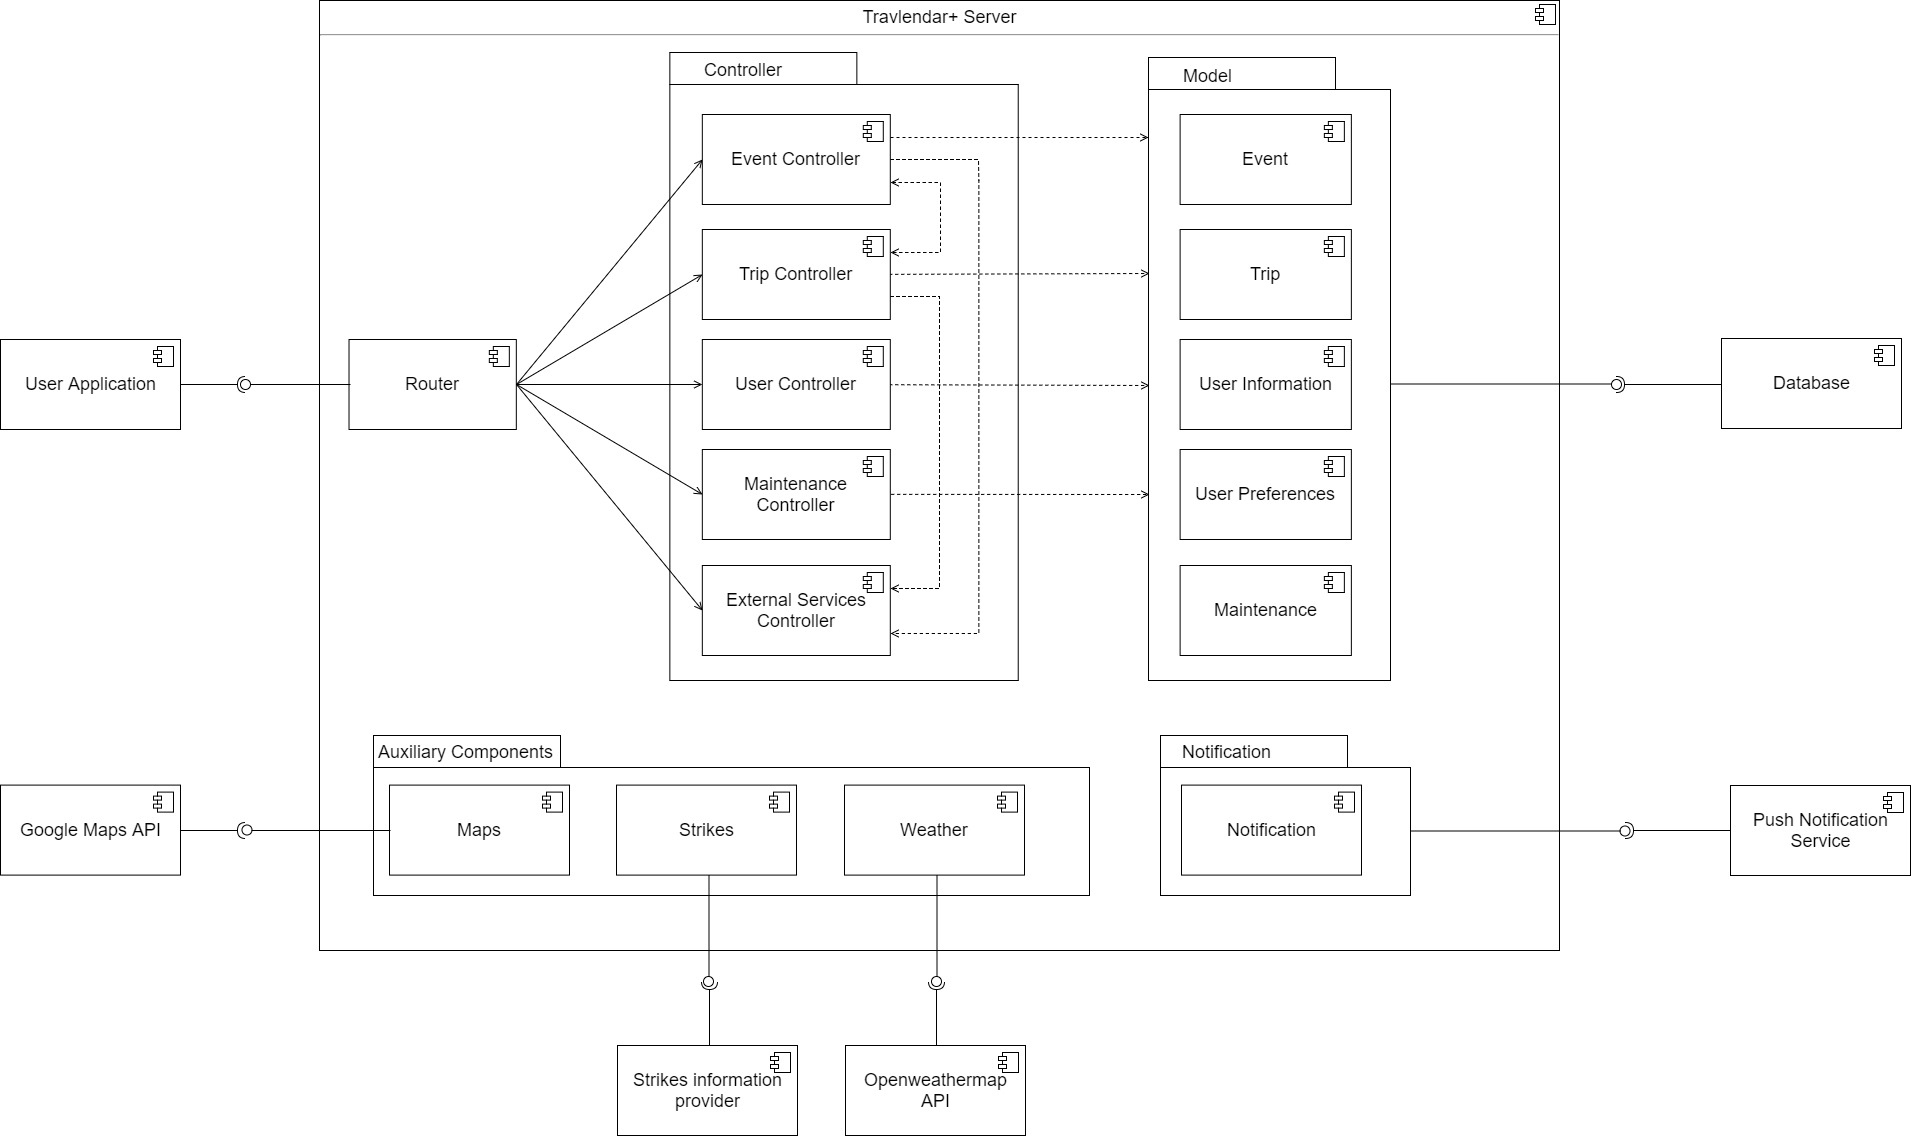
\includegraphics[width=1.47\textwidth]{MainMatter/images/ad/component}}
\captionof{figure}{Component View of the system}
\end{center}
\end{landscape}

%
% ------------------------------------------------------------------------ %
%
\section{Deployment View}
%
% ------------------------------------------------------------------------ %
%
\section{Runtime View}
In this section some sequence diagrams will be presented to describe the interactions that happen between the main components of the system when the most common functionalities are used. This is a high-level description of the actual interactions of the system-to-be, so functions and their names may be added, modified or deleted during the development process.

\pagebreak
\begin{landscape}
\begin{center}
\thispagestyle{empty}
\makebox[\textwidth][c]{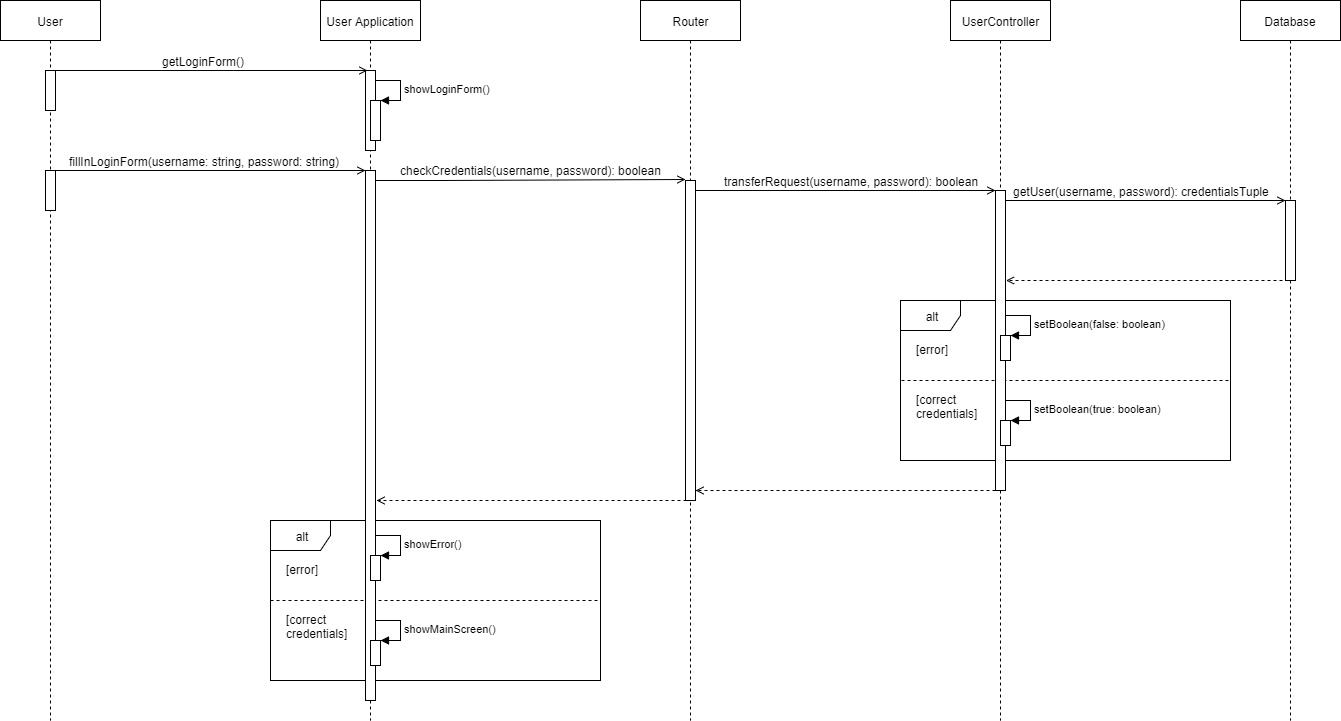
\includegraphics[width=1.76\textwidth]{MainMatter/images/runtime/login}}
\captionof{figure}{User Login runtime view}
\end{center}
\end{landscape}

\pagebreak
\begin{landscape}
\begin{center}
\thispagestyle{empty}
\makebox[\textwidth][c]{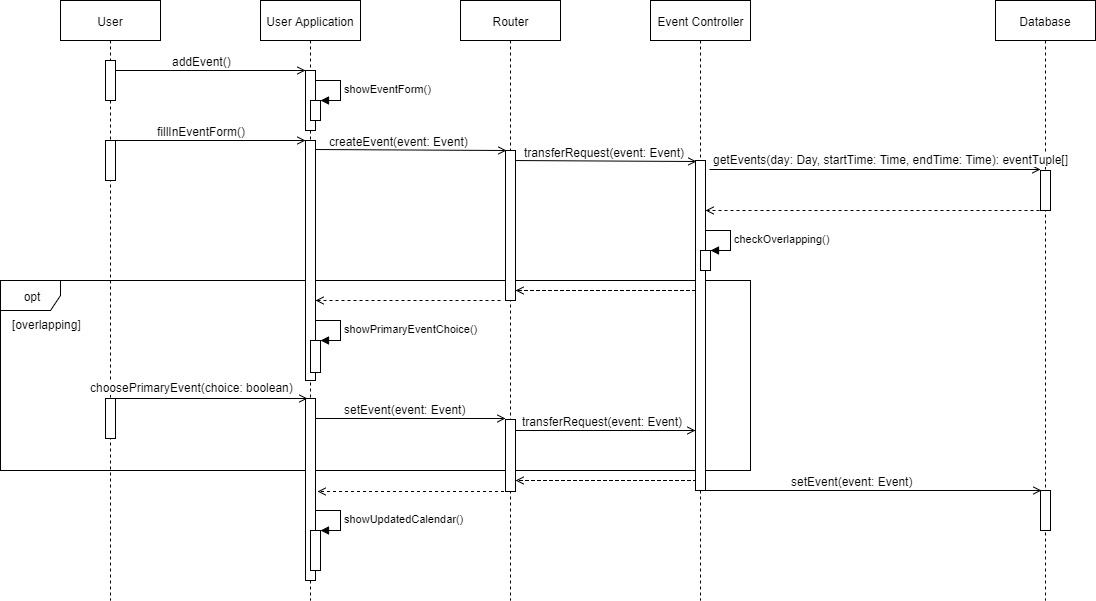
\includegraphics[width=1.72\textwidth]{MainMatter/images/runtime/add}}
\captionof{figure}{Adding of an event in the calendar runtime view}
\end{center}
\end{landscape}

\pagebreak
\begin{landscape}
\begin{center}
\thispagestyle{empty}
\makebox[\textwidth][c]{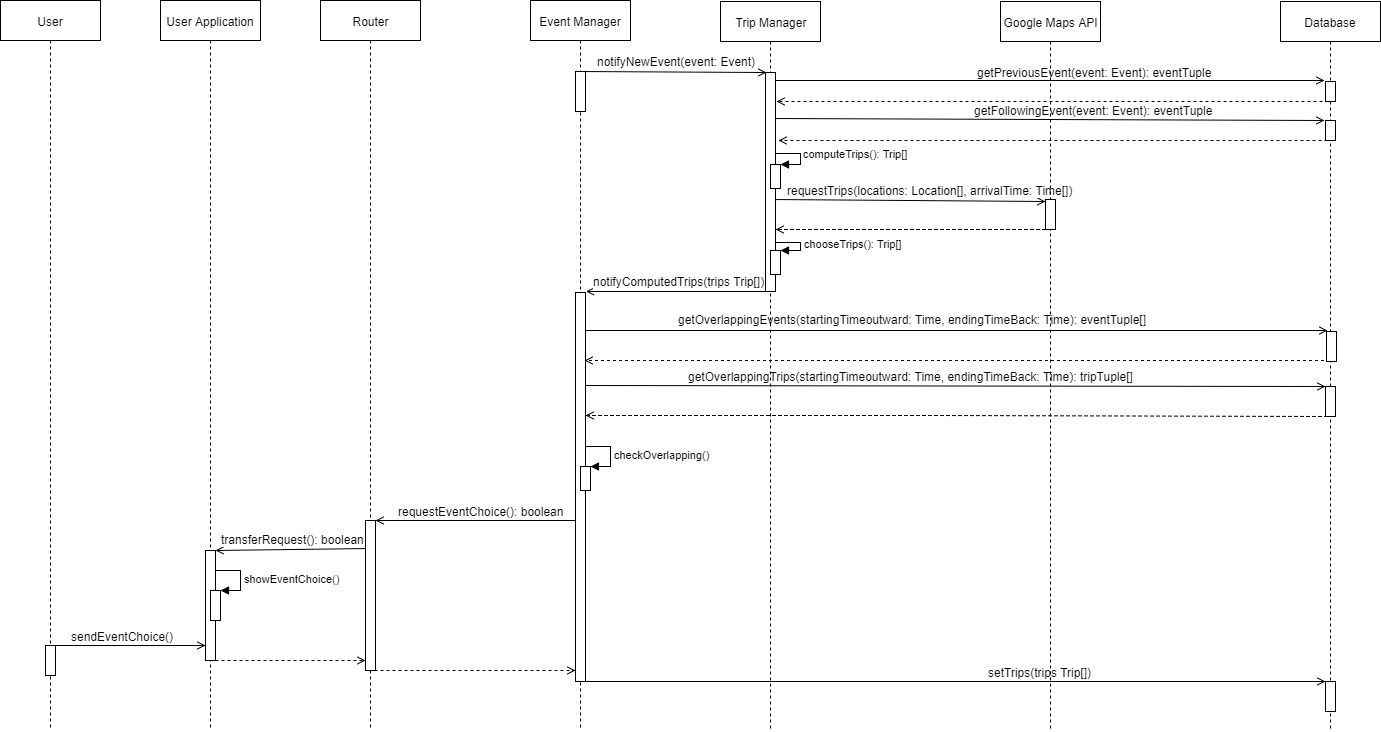
\includegraphics[width=1.78\textwidth]{MainMatter/images/runtime/tripcomm}}
\captionof{figure}{Trip planning runtime view}
\end{center}
\end{landscape}

\pagebreak
\begin{landscape}
\begin{center}
\thispagestyle{empty}
\makebox[\textwidth][c]{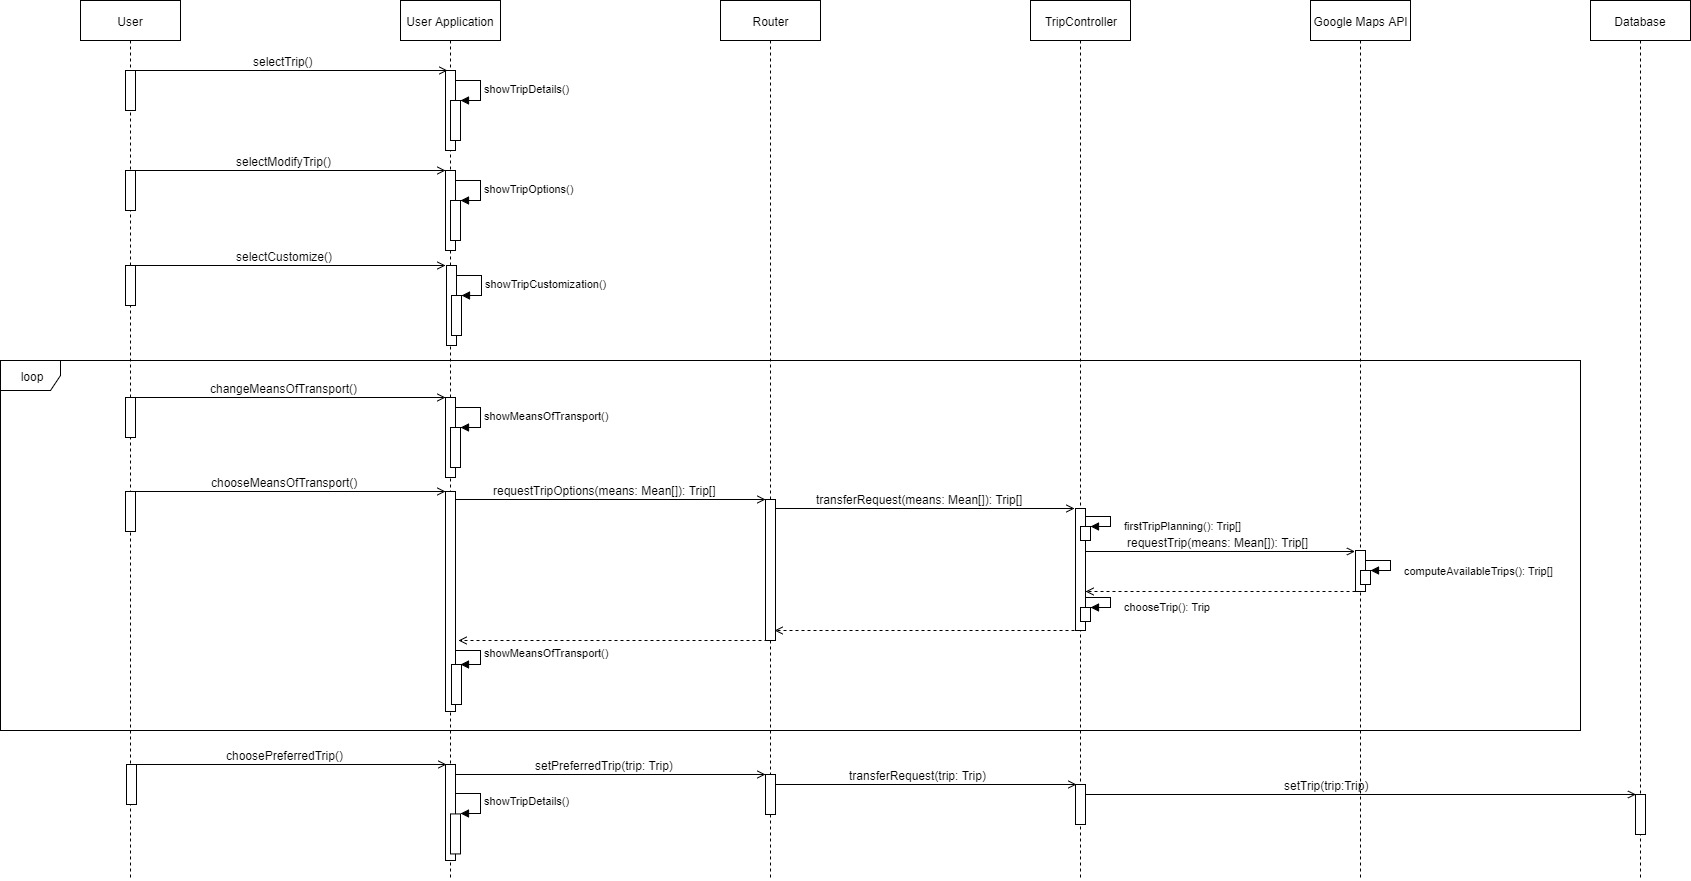
\includegraphics[width=1.81\textwidth]{MainMatter/images/runtime/tripcustom}}
\captionof{figure}{Trip customization runtime view}
\end{center}
\end{landscape}
%
% ------------------------------------------------------------------------ %
%
\section{Component Interfaces}
%
% ------------------------------------------------------------------------ %
%
\section{Selected Architectural Styles and Patterns}
%
% ------------------------------------------------------------------------ %
%
\section{Other Design Decisions}
%
%
% -----------------------------END------------------------------------- %